\documentclass[a4paper]{article}

\usepackage[T1]{fontenc}
\usepackage{graphicx}
\usepackage{amsmath}
\usepackage[utf8]{inputenc}
\usepackage{enumitem}
\setlist[description]{style=unboxed}

\usepackage{tikz}
\usepackage{pgfplots}
\usepackage{circuitikz}
\usepackage{tabularx}

\usetikzlibrary{calc,positioning,shapes,decorations.pathreplacing}

\tikzset{
	short/.style={draw,rectangle,text height=3pt,text depth=13pt,
		text width=7pt,align=center,fill=gray!30},
	long/.style={short,text width=1.5cm},
	verylong/.style={short,text width=4.5cm}
}

\begin{document}
\section{AC voltage rectifier and regulator}

\subsection{Introduction}

For fully functional operation, submarine/robot arm/habitat is equipped with 
lot of computer based subsystems and electronic devices which operate on DC 
voltage. To ensure proper operation the DC voltage has to be stable and without 
noise.

To ensure stable DC voltage, linear regulator on Fig. 1. is used. Due to 
extreme conditions in the system, regulators often fail and components have to 
be repaired or replaced with proper spare part.

In this task, your job is to:
\begin{itemize}
\item identify components that failed in different scenarios, 
\item find the proper replacement parts, 
\item ensure that the output voltage ripple is within the boundaries with 
proper low pass filter,
\item find the probability of future malfunction in standby redundant system.
\end{itemize}

\begin{figure}[h!]
\centering
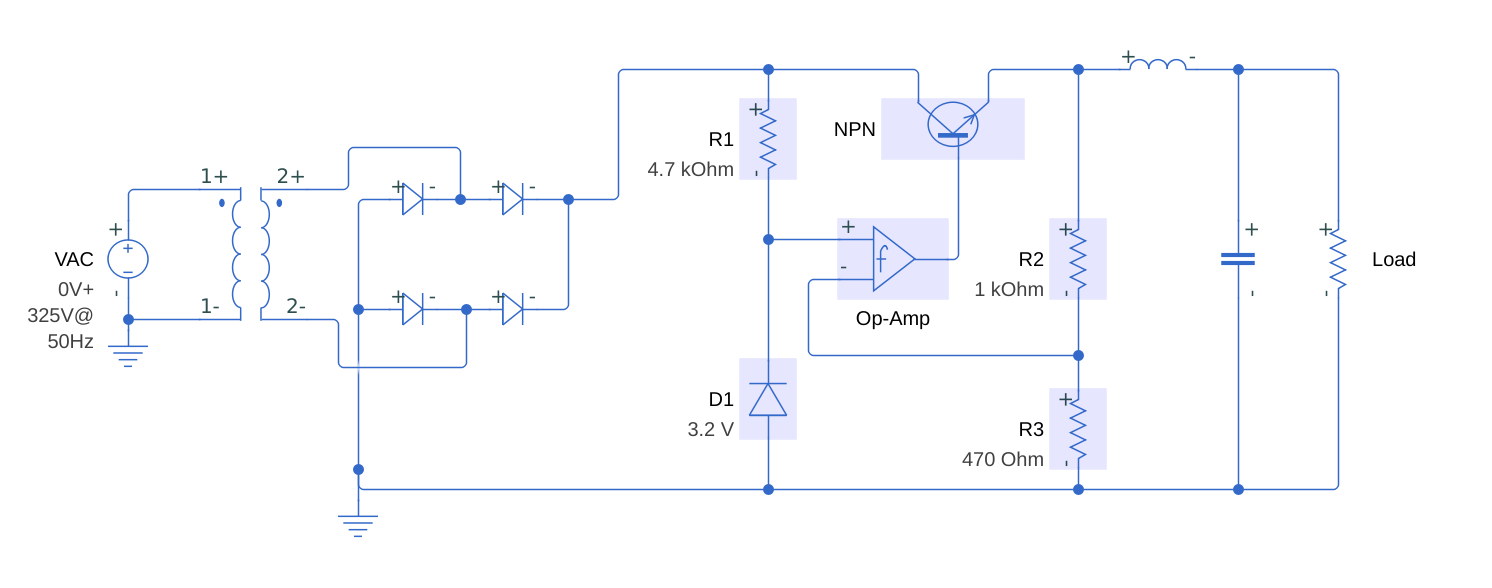
\includegraphics[width=\linewidth]{images/reg.png}

\caption{Rectifier and linear regulator.}
\end{figure}

\textbf{Regulator specifications.} Regulator specifications are provided with 
the following table. In each task you have to ensure that the values specified
in the table correspond to the values which will be measured in simulation. 

\begin{table}[h!]
    \hyphenpenalty 10000
    \caption{Regulator specifications}
    \label{tab:spec}
    \begin{tabularx}{\linewidth}{|X|X|X|X|} \hline
    PARAMETER & TEST CONDITIONS & VALUE & UNIT \\ \hline 
    Output voltage ($V_o$)& $I_o = 1$ A & $12.00$ & V \\ \hline
    Output current ($I_o$) & a & $1.5$ & A \\ \hline
    Ripple rejection & (50 Hz) & $78$ & dB \\ \hline
   	Dropout voltage & $I_o = 1.5$ A & $2$ & V \\ \hline
    \end{tabularx}
\end{table}

\subsection{Identifying failed components and replacement}

Each failure is described with a set of time diagrams in specific test points 
which can be seen on regulator schematic document. Based on the provided 
diagrams you have to determine which component failed. In each failure scenario
only one component is broken. There are three different failure scenarios which
are described below. First of, figures of test points correct operation are 
given with figures Fig. \ref{fig:correct1} - \ref{fig:correctN}. After you 
detect failure the component will be replaced with appropriate component from
stash. For each part of the task you need to provide designator of broken 
component. 

\textbf{1. failure scenario} %%- Zener diode}

\textbf{2. failure scenario}  %%- Diode in rectifier bridge}

\subsection{Choosing replacement components}

In previous task, you had to identify malfunction in linear regulator circuit.
Now, with given broken component you have to find appropriate component in 
stash. As a supplier use DigiKey Electronics. Your choice is graded in 
several ways:
\begin{itemize}
\item price,
\item correct voltage, power and current ratings,
\item correct component footprint.
\end{itemize}
As a result, please provide DigiKey part number for each scenario.

\textbf{1. scenario - Resistor (R1)}

\textbf{2. scenario - Transistor (Q1)}

\subsection{LC filter design}

To achieve specified ripple rejection at required frequency, design a LC low 
pass filter which filters output of regulator. As in previous task you have 
to provide to DigiKey part numbers for LC filter. Your choice is graded in 
the similar fashion as before:
\begin{itemize}
\item price,
\item correct inductance and capacitance,
\item correct footprints, 
\item correct current and voltage ratings.
\end{itemize}

\subsection{Reliability of a standby system}


\subsection{Grading scheme}
 
\end{document}